\documentclass[10pt,english,a4paper]{article}
\usepackage[utf8]{inputenc}
\usepackage{graphicx}
\usepackage{url} 
\usepackage{hyperref} 
\usepackage{cite}
\pagestyle{headings}


\title{Improving computer science and software 
engineering education in cyberlearning 
environments through understanding UI and UX design
\thanks{Semestrálny projekt v predmete Metódy inžinierskej práce,
 ak. rok 2020/21, vedenie: Martin Sabo}}

\author{Márk Bartalos \\[2pt]
        \small{Slovak University of Technology in Bratislava}\\
        \small{Faculty of Informatics and Information Technologies}\\
        \small{\texttt{xbartalosm@stuba.sk}}
}


\begin{document}

\maketitle

\begin{abstract}
    In our day and age cyberlearning for computer science and software engineering education has become more popular than ever.
    Thanks to its growing popularity and adoption rate, online cyberlearning environments (CLE) are advancing very quickly.
    In order to make these CLEs as effective and user-friendly as possible, we need to understand how their design
    works and what common problems can occur. This article will offer possible testing solutions for analyzing and testing
    the design of complex CLEs and web tools targeted for computer science (CS) and software engineer (SE) students. 
    It will give a better understanding what exactly is meant under the terms ``UI/UX", will include an analysis of
    popular online CLEs, which can serve as a pointer for improving these environments, which will in a way improve teaching these fields.
    
\end{abstract}



\section{Introduction}
We speak about distance learning from around two centuries ago, under which
I am referring to learning through online environments\cite{moore_2011_elearning}. What distance learning really means is highly debated,
but I believe it can also refer to learning through online environments, because lot of authors use learning through an online environment and distance learning as
synonyms\cite{moore_2011_elearning}\cite{distance_definition}. 
\paragraph{Technology and people}
Cyberlearning seems as a very promising technology for helping us in learning and in the automatization of the learning
experience. It has a potential to revolutionize how we learn today, be replacing face to face learning with
learning through technology.

Now distance learning is becoming a necessity rather than an option. Especially in the middle of a pandemic, use of online 
education environments have become more needed than ever. This article will focus on online cyberlearning environments 
mainly designed for computer science (CS) and software engineer (SE) students.


\section*{Contents}

\begin{itemize}
     \item The used terms will be defined in the definitions section \ref{definitions}.
     \item Methods that could be used will be explored more in section ``Methods for analysis" \ref{methods}.
     \item I will have an analysis of the most commonly used environments in the section `` Analysis of popular environments" \ref{analysis}.
\end{itemize}


\section{Definitions}\label{definitions}

\subsection{Cyberlearning}
For cyberlearning I will use the definition by National Science Foundation: 
``the use of networked computing and communications technologies to support learning” \cite{borgman_2017_fostering} 
Cyberlearning itself can be form of distance learning, but its main focus is building an all 
encompassing online environment which can motivate, inspire and and teach students using 
computer systems and networking technologies as primary tools\cite{ui/ux}.
Primary goal of cyberlearning is to provide learning experiences via a technology-based platform. 
Cyberlearning in some way is an extension of and a twist on e-learning \cite{lynch_2020_cyberlearning}.
While e-learning refers to how the content is delivered, in cyberlearning, technology
is used to carry out learning experiences which would be otherwise impossible without technology \cite{lynch_2020_cyberlearning}.

\subsection{Cyberlearning env. for CS and SE students}
Under the term ``Cyberlearning environments for computer science and software engineer students", I am mainly
referring to an online CLE which enable students to write and compile code online. These are all encompassing
environments, meaning they are equipped with 
online compilers and debugging tools, so students don't require any additional software to be installed on their PC, making
the whole programming experience more accessible for everyone.
With the help of these kind of CLEs students are able to learn the curriculum through lectures and practice
what they have learnt, with only requiring a web browser.

\subsection{User Interface (UI)}
UI and UX are often confused terms\cite{theymakedesign_2019_what}. They have similarities, but in reality
these are completely different things.
UI stands for User Interface. User Interface design defines the graphical layout of the page or application.
User interface designers are responsible for defining the how each element will look, their size and position.
Its their job to make the look and feel of the page or application aesthetically pleasing and 
attractive. Animation, transition design, choosing of the correct fonts and images also part of the UI design, 
these have to be designed such a way that they are in harmony and logically connected to each other\cite{theymakedesign_2019_what}.


\subsection{User Experience (UX)}
UX stands for ``user experience". UX designers are also concerned with the user interface\cite{theymakedesign_2019_what}. 
The main difference between UI and UX is that while UI focuses on the look of the application,
UX focuses on the functionality and interactions of the application. UX designers are 
responsible form making sure the user experience is intuitive and can be easily understood by everyone.
They have to make sure that the connection between different parts are organized in a logical way.
UX designers are also have to have an understanding of how users interact with their
device so that the UX can be easy to use and user friendly\cite{theymakedesign_2019_what}. 

\section{Importance of UI/UX design}\label{importance}
UI is the interface between the user and the functionality of the application. UI and UX are responsible for
how the content is presented, how the navigation works, how the different interactions behave. It 
has complete control over what the users sees.

\paragraph{Graphical expression of information}
It is very important how we present the information. Graphical expression of information is on of the best methods of presentation. CLEs can be
a great tool for graphically presenting data. There is difference even in two graphical presentations,
that is why we have to pay attention to how is the UI of the presentation designed and implemented. 


Design of the environment has a big role in the effectiveness and in 
its ability to properly convey information \cite{ui/ux}. 
By a study done in 2002 called "Usability evaluation of web-based learning", we know that User interface
has reasonable impact on the student's behavior while using the environment\cite{wesson_2002_usability}.
The study concluded that students preferred the environment which provided a consistent experience and could be more easily navigated 
\cite{wesson_2002_usability}. That is why its necessary to create CLEs that can be easily navigated,
where information and tools are arranged into logical groups and have a consistent user-friendly design.

\begin{figure}[h]
    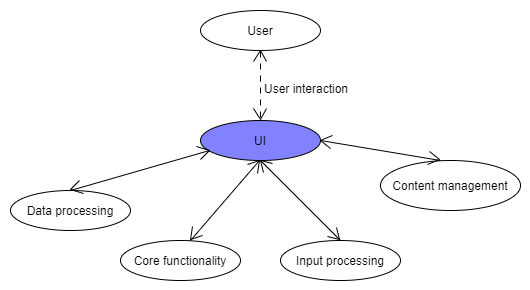
\includegraphics[width=1\textwidth]{images/ui-diagram2.png}
    \caption{Diagram illustrating the role of UI in CLE}
\end{figure}


\section{Methods for analysis}\label{methods}
There are several methods for testing UI/UX design of online environments. The testing 
can be automated or done by a group of people manually.

\subsection{Heuristic evaluation}
Heuristic evaluation of the interface can be done by one person, but
its not recommended because one person will never be able to
find all the problems, so it is usually done by a group of people\cite{a2020_heuristic}. 
The result of six studies shows that the number of errors spotted is proportional to the number of evaluators,
meaning that with the increase in the number of evaluators, precision of the evaluation increases, see Figure~\ref{fig:increase}.
Heuristic evaluation consists of each individual inspecting the interface alone. Only after the
inspection are they allowed to communicate with each other or have their findings aggregated\cite{a2020_heuristic}.
This method can be used even when the user doesn't know anything about the user interface by
the help of an observer. In this case the observer's job is to record the comments of the evaluator\cite{a2020_heuristic}.

\begin{figure}[h]
    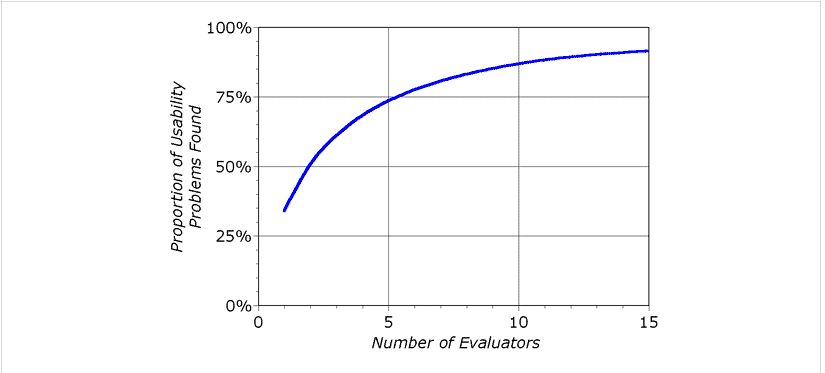
\includegraphics[width=1\textwidth]{images/heuristic-results.png}
    \caption{Curve showing the proportion of usability problems in an interface
     found by heuristic evaluation using various numbers of evaluators\cite{a2020_heuristic}.}
     \label{fig:increase}
\end{figure}
The output of using heuristic evaluation are problems with the interface with reference to the usability
principles that were violated\cite{a2020_heuristic}. Because the concreteness of the output 
its easier and faster to develop a solution for these problems. 



\subsection{Automated testing}
Automated testing of UI is a relatively new thing\cite{automated_testing_ifml}. There aren't many well known methods
providing fully automatic testing of a web environment, but a recent study has shown that
it is possible using Interaction Flow Modeling Language (IFML) Models\cite{automated_testing_ifml}.
IFML is evolved from WebML and its designed to capture the structure, user interaction and control
flow of front-end of web applications\cite{automated_testing_ifml}.


\paragraph{Content modelling}
To automate and validate the UI design the developers have to create an IFML model
of the front-end. In order to design an IFML model, an UML (Universal Modelling Language) model 
containing the domain concepts of the application is required\cite{automated_testing_ifml}. 
When the IFML and the UML models are completed they have to be processed by an application written 
in Java, which will generate a Test case document (.txt), a Navigation Modell (.xta) and a State Transition 
Matrix (.xls). Then the generated data can be used to analyze and easily spot flaws with the web application, like bad navigation design
\cite{automated_testing_ifml}. 
Thanks to usage of generalized Markup Languages this application can be used for all kind of web environments. 
By using this program we could analyze our web based CLEs for CS and SE students. 
The produced data then could be used to improve their layout, remove confusing elements and improve the usability of the design,
making the learning process more efficient.


\section{Analysis of popular environments}\label{analysis}
The alaysis was done on the following online environments: Udemy, Skillshare, Freecodecamp, Treehouse.
The analysis was done by myself due to lack of resources for hiring a professional team. The results are integer values
from 1-10 where 10 is the best and 1 is the worst. The produced data is not as accurate as it was done
by a professional testing team, it can be subjective, but it should serve as a general pointer for
how these online CLEs compare to each other.

% Please add the following required packages to your document preamble:

\begin{center}
    \begin{tabular}{|l|l|l|l|l|}
    \hline
                            & \textbf{Udemy} & \textbf{Skillshare} & \textbf{Freecodecamp} & \textbf{Treehouse} \\ \hline
    Overall usability       & 8              & 10                  & 5                     & 9                  \\ \hline
    Design intuitivness     & 6              & 10                  & 5                     & 10                 \\ \hline
    Navigation layout       & 8              & 9                   & 6                     & 8                  \\ \hline
    Inform. arrangement     & 8              & 10                  & 6                     & 9                  \\ \hline
    \textbf{Total}          & 30             & 39                  & 22                    & 36                 \\ \hline
    \end{tabular}
\end{center}


\section{Conclusion}
The currently available online CLEs can be a great tool for improving the learning process, but for 
them to do that they need to be implemented correctly, they have to be easy to use and compatible 
with most of the popular browsers. Our analysis shows that most of the popular ones are
implemented well. Most of them had a well designed navigation layout, the information were arranged
in a way that everything could be found easily and all of them were easy to use.   

\subsection*{Testing}
There is a growing need of development in testing of these web based learning environments, in order
to improve them and make the learning experience more effective.
Although there are solutions for automatically analyzing web applications, this technology is still work
in progress. Manual heuristic analysis can be done by everyone, but the results will not be as precise as
in a case done by a professional or by multiple people. For precise data more people is needed.




\bibliography{citations}
\bibliographystyle{ieeetr}
\end{document}
